\documentclass[main.tex]{subfiles}                                              

\begin{document}

\section{引言}

在本章中，我们结合了第 1 章第 1.4 节和 1.5 节的概念以及第 3 章的内容，以获得非均匀有理 B-样条(NURBS)曲线和曲面。我们给出定义和一般性质，并推导出 NURBS 曲线和曲面的导数的公式和算法，这些导数以其非有理对应物为基础。关于 NURBS 的最早出版作品是 [Vers75; Till83]。更近期的综述可以在 [Pieg91a] 中找到。

\section{NURBS曲线的定义与性质}

一个 \(p\) 次 NURBS 曲线定义为

\[
\mathbf{C}\left( u\right)  = \frac{\mathop{\sum }\limits_{{i = 0}}^{n}{N}_{i,p}\left( u\right) {w}_{i}{\mathbf{P}}_{i}}{\mathop{\sum }\limits_{{i = 0}}^{n}{N}_{i,p}\left( u\right) {w}_{i}}\;a \leq  u \leq  b \tag{4.1}
\]

其中 \(\left\{  {\mathbf{P}}_{i}\right\}\) 是控制点(形成控制多边形)， \(\left\{  {w}_{i}\right\}\) 是权重， \(\left\{  {{N}_{i,p}\left( u\right) }\right\}\) 是在非周期(且非均匀)节点向量上定义的 \(p\) 次 B-样条基函数。

\[
U = \left\{  {\underset{p + 1}{\underbrace{a,\ldots ,a}},{u}_{p + 1},\ldots ,{u}_{m - p - 1},\underset{p + 1}{\underbrace{b,\ldots ,b}}}\right\}
\]

除非另有说明，我们假设 \(a = 0,b = 1\) 和 \({w}_{i} > 0\) 对所有 \(i\) 成立。设定

\[
{R}_{i,p}\left( u\right)  = \frac{{N}_{i,p}\left( u\right) {w}_{i}}{\mathop{\sum }\limits_{{j = 0}}^{n}{N}_{j,p}\left( u\right) {w}_{j}} \tag{4.2}
\]

允许我们将方程 (4.1) 重写为以下形式

\[
\mathbf{C}\left( u\right)  = \mathop{\sum }\limits_{{i = 0}}^{n}{R}_{i,p}\left( u\right) {\mathbf{P}}_{i} \tag{4.3}
\]

\(\left\{  {{R}_{i,p}\left( u\right) }\right\}\) 是有理基函数；它们是在 \(u \in  \left\lbrack  {0,1}\right\rbrack\) 上的分段有理函数。

\({R}_{i,p}\left( u\right)\) 具有以下从方程 (4.2) 及其对应的 \({N}_{i,p}\left( u\right)\) 性质推导出的特性:

P4.1 非负性:对于所有 \(i,p\) 和 \(u \in  \left\lbrack  {0,1}\right\rbrack\) ，有 \({R}_{i,p}\left( u\right)  \geq  0\) ；

P4.2 单位分割:对于所有 \(u \in  \left\lbrack  {0,1}\right\rbrack\) ，有 \(\mathop{\sum }\limits_{{i = 0}}^{n}{R}_{i,p}\left( u\right)  = 1\) ；

P4. \(3{R}_{0,p}\left( 0\right)  = {R}_{n,p}\left( 1\right)  = 1\) ;

P4.4 对于 \(p > 0\) ，所有 \({R}_{i,p}\left( u\right)\) 在区间 \(u \in  \left\lbrack  {0,1}\right\rbrack\) 上恰好达到一个最大值。

P4.5 局部支持:对于 \(u \notin  \left\lbrack  {{u}_{i},{u}_{i + p + 1}}\right)\) ，有 \({R}_{i,p}\left( u\right)  = 0\) 。此外，在任何给定的节点区间内，最多有 \(p + 1\) 个 \({R}_{i,p}\left( u\right)\) 是非零的(一般情况下， \(\left. {{R}_{i - p,p}\left( u\right) ,\ldots ,{R}_{i,p}\left( u\right) \text{ are nonzero in }\left\lbrack  {{u}_{i},{u}_{i + 1}}\right) }\right)\) ；

P4.6 所有 \({R}_{i,p}\left( u\right)\) 的导数在节点区间的内部存在，在那里它是一个具有非零分母的有理函数。在节点处， \({R}_{i,p}\left( u\right)\) 是 \(p - k\) 次连续可微的，其中 \(k\) 是节点的重数；

P4.7 如果对于所有 \(i\) 有 \({w}_{i} = 1\) ，那么对于所有 \(i\) 有 \({R}_{i,p}\left( u\right)  = {N}_{i,p}\left( u\right)\) ；即， \({N}_{i,p}\left( u\right)\) 是 \({R}_{i,p}\left( u\right)\) 的特例。实际上，对于任何 \(a \neq  0\) ，如果对于所有 \(i\) 有 \({w}_{i} = a\) ，那么对于所有 \(i\) 有 \({R}_{i,p}\left( u\right)  = {N}_{i,p}\left( u\right)\) 。

性质 P4.1-P4.7 产生了 NURBS 曲线的以下重要几何特征:

P4.8 \(\mathbf{C}\left( 0\right)  = {\mathbf{P}}_{0}\) 和 \(\mathbf{C}\left( 1\right)  = {\mathbf{P}}_{n}\) ；这由 P4.3 推导而来；

P4.9 仿射不变性:通过对控制点应用仿射变换来对曲线施加仿射变换(见 P3.4，第 3.1 节)；NURBS 曲线在透视投影下也是不变的([Lee87; Pieg91a])，这一事实在计算机图形学中非常重要；

P4.10 强凸包性质:如果 \(u \in  \left\lbrack  {{u}_{i},{u}_{i + 1}}\right)\) ，则 \(\mathbf{C}\left( u\right)\) 位于控制点 \({\mathbf{P}}_{i - p},\ldots ,{\mathbf{P}}_{i}\) 的凸包内(见图 4.1，其中 \(\mathbf{C}\left( u\right)\) 对于 \(u \in  \left\lbrack  {1/4,1/2}\right)\) (虚线段)包含在凸包内)；

\begin{center}
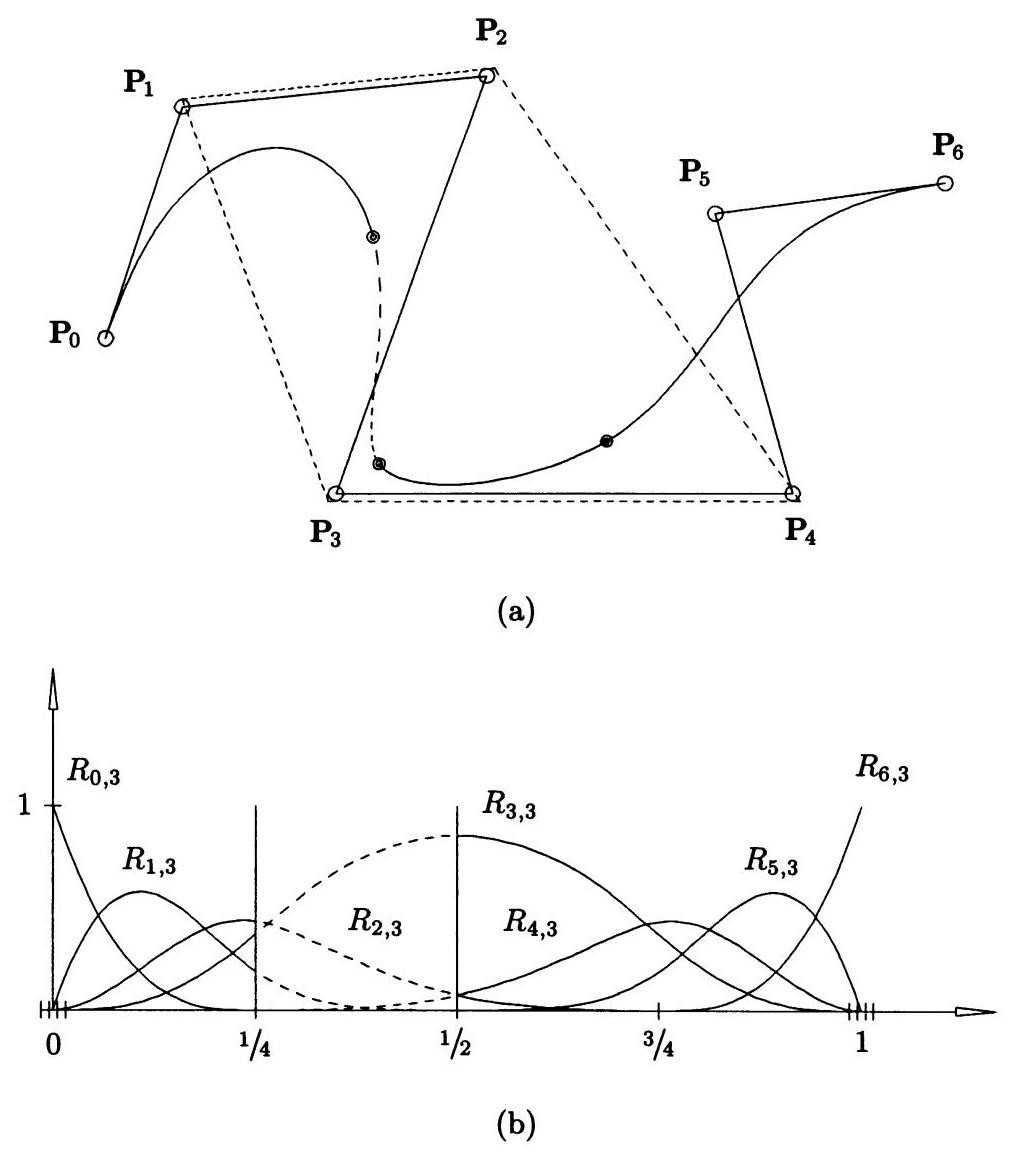
\includegraphics[max width=0.9\textwidth]{images/0193ba0d-ab19-7138-9798-cb281ce60de0_129_260_246_1009_1154_0.jpg}
\end{center}
\hspace*{3em} 

图 4.1. \(U = \{ 0,0,0,0,1/4,1/2,3/4,1,1,1,1\}\) 和 \(\left\{  {{w}_{0},\ldots ,{w}_{6}}\right\}   = \{ 1,1,1,3,1,1,1\}\) 。(a) 一条三次 NURBS 曲线；(b) 相关的基函数。

\(\left\{  {{\mathbf{P}}_{1},{\mathbf{P}}_{2},{\mathbf{P}}_{3},{\mathbf{P}}_{4}}\right\}\) 的虚线区域)；这由 P4.1、P4.2 和 P4.5 推导而来；

P4.11 \(\mathbf{C}\left( u\right)\) 在节点跨度的内部是无限可微的，并且在重数为 \(k\) 的节点处是 \(p - k\) 次可微的；

P4.12 变化减小性质:没有平面与曲线的交点比与控制多边形的交点更多(对于二维曲线，将“平面”一词替换为“直线”)；

P4.13 没有内部节点的 NURBS 曲线是有理 Bézier 曲线，因为 \({N}_{i,p}\left( u\right)\) 简化为 \({B}_{i,n}\left( u\right)\) ；将方程 (4.2) 和 (4.3) 与方程 (1.15) 进行比较。这与 P4.7 一起，意味着 NURBS 曲线包含非有理 B-样条和有理及非有理 Bézier 曲线作为特例；

P4.14 局部近似:如果控制点 \({\mathbf{P}}_{i}\) 被移动，或者权重 \({w}_{i}\) 被改变，它只影响区间 \(u \in  \left\lbrack  {{u}_{i},{u}_{i + p + 1}}\right)\) 上曲线的那一部分；这遵循于 P4.5。

性质 P4.14 对于交互式形状设计非常重要。使用 NURBS 曲线，我们可以利用控制点移动和权重修改来实现局部形状控制。图 4.2-4.6 显示了修改单个权重的效果。定性效果是:假设 \(u \in  \left\lbrack  {{u}_{i},{u}_{i + p + 1}}\right)\) ；那么如果 \({w}_{i}\) 增加(减少)，点 \(\mathbf{C}\left( u\right)\) 会更靠近(远离) \({\mathbf{P}}_{i}\) ，因此曲线被拉向(推离) \({\mathbf{P}}_{i}\) 。此外，对于固定的 \(u\) ， \(\mathbf{C}\left( u\right)\) 的移动沿着一条直线(图 4.6)。在图 4.6 中， \(u\) 固定而 \({w}_{3}\) 变化。让

\[
\mathbf{B} = \mathbf{C}\left( {u;{w}_{3} = 0}\right)  \tag{4.4}
\]

\[
\mathbf{N} = \mathbf{C}\left( {u;{w}_{3} = 1}\right)
\]

然后由 \(\mathbf{B}\) 和 \(\mathbf{N}\) 定义的直线通过 \({\mathbf{P}}_{3}\) ，对于任意的 \(0 < {w}_{3} < \infty ,{\mathbf{B}}_{3} = \mathbf{C}\left( {u;{w}_{3}}\right)\) ，它位于 \(\mathbf{B}\) 和 \({\mathbf{P}}_{3}\) 之间的这条线段上。我们将在后面的章节中回到这个主题。

与有理 Bézier 曲线一样，同质坐标提供了一种有效的方法来表示 NURBS 曲线。设 \(H\) 为由方程 (1.16) 给出的透视映射。对于给定的一组控制点 \(\left\{  {\mathbf{P}}_{i}\right\}\) 和权重 \(\left\{  {w}_{i}\right\}\) ，构造加权控制点 \({\mathbf{P}}_{i}^{w} = \left( {{w}_{i}{x}_{i},{w}_{i}{y}_{i},{w}_{i}{z}_{i},{w}_{i}}\right)\) 。然后在四维空间中定义非有理(分段多项式)B-spline 曲线为

空间为

\[
{\mathbf{C}}^{w}\left( u\right)  = \mathop{\sum }\limits_{{i = 0}}^{n}{N}_{i,p}\left( u\right) {\mathbf{P}}_{i}^{w} \tag{4.5}
\]

\begin{center}
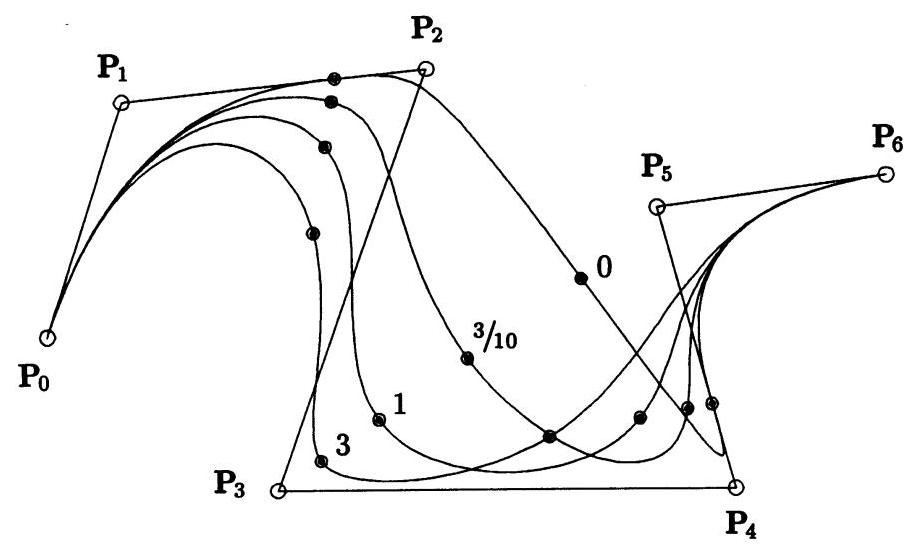
\includegraphics[max width=0.8\textwidth]{images/0193ba0d-ab19-7138-9798-cb281ce60de0_130_313_1513_911_549_0.jpg}
\end{center}
\hspace*{3em} 

图 4.2. 有理三次 B-spline 曲线，随着 \({w}_{3}\) 的变化。

\begin{center}
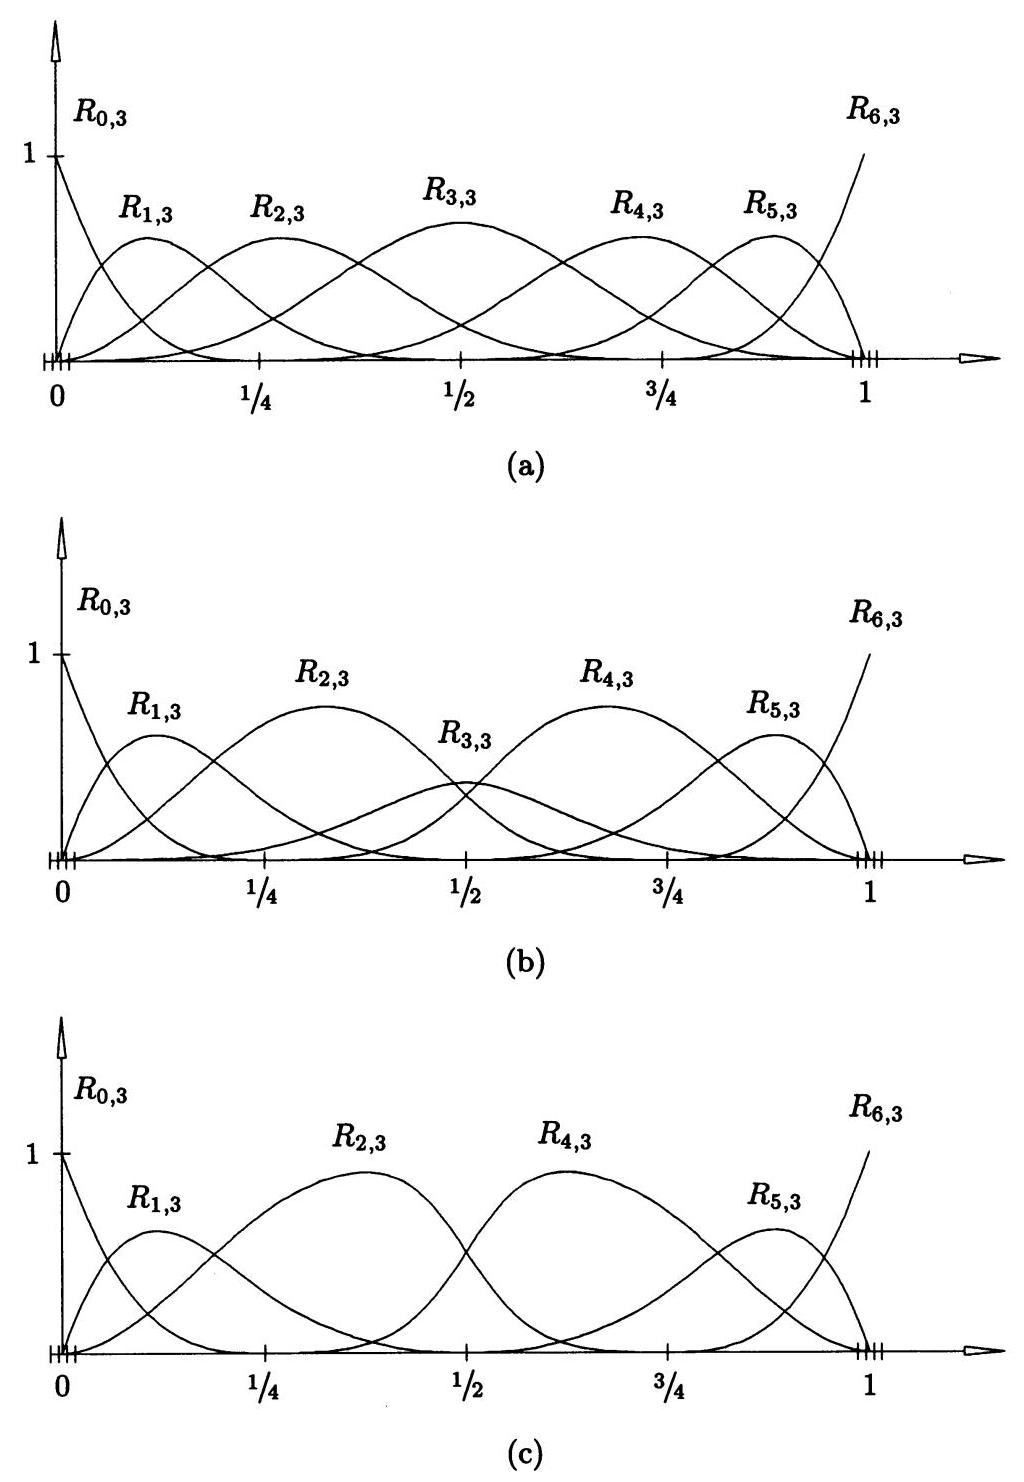
\includegraphics[max width=0.9\textwidth]{images/0193ba0d-ab19-7138-9798-cb281ce60de0_131_251_295_1024_1482_0.jpg}
\end{center}
\hspace*{3em} 

图 4.3. 图 4.2 曲线的立方基函数。(a) \({w}_{3} = 1\) ; (b) \({w}_{3} = 3/{10};\left( \mathrm{c}\right) {w}_{3} = 0.\)

应用透视映射 \(H\) 到 \({\mathbf{C}}^{w}\left( u\right)\) 产生相应的有理 B 样条曲线(在三维空间中分段有理)

\[
\mathbf{C}\left( u\right)  = H\left\{  {{\mathbf{C}}^{w}\left( u\right) }\right\}   = H\left\{  {\mathop{\sum }\limits_{{i = 0}}^{n}{N}_{i,p}\left( u\right) {\mathbf{P}}_{i}^{w}}\right\}
\]

\[
= \frac{\mathop{\sum }\limits_{{i = 0}}^{n}{N}_{i,p}\left( u\right) {w}_{i}{\mathbf{P}}_{i}}{\mathop{\sum }\limits_{{i = 0}}^{n}{N}_{i,p}\left( u\right) {w}_{i}} = \mathop{\sum }\limits_{{i = 0}}^{n}{R}_{i,p}\left( u\right) {\mathbf{P}}_{i}
\]

\begin{center}
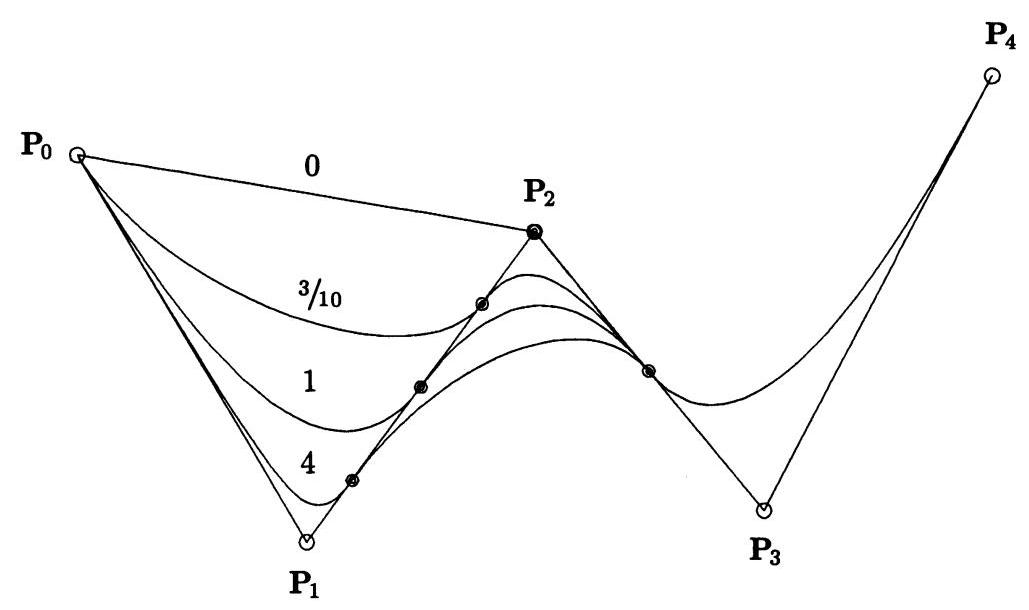
\includegraphics[max width=0.9\textwidth]{images/0193ba0d-ab19-7138-9798-cb281ce60de0_132_256_271_1029_610_0.jpg}
\end{center}
\hspace*{3em} 

图 4.4. 有理二次曲线，具有变化的 \({w}_{1}\) 。

我们可以交替地将 \({\mathbf{C}}^{w}\left( u\right)\) 或 \(\mathbf{C}\left( u\right)\) 称为 NURBS 曲线，尽管严格来说， \({\mathbf{C}}^{w}\left( u\right)\) 不是一条有理曲线。

\section*{示例}

Ex4.1 设 \(U = \{ 0,0,0,1,2,3,3,3\} ,\left\{  {{w}_{0},\ldots ,{w}_{4}}\right\}   = \{ 1,4,1,1,1\} ,\left\{  {{\mathbf{P}}_{0},\ldots ,{\mathbf{P}}_{4}}\right\}\)  \(= \{ \left( {0,0}\right) ,\left( {1,1}\right) ,\left( {3,2}\right) ,\left( {4,1}\right) ,\left( {5, - 1}\right) \}\) 。我们计算在 \(u = 1\) 处的有理 B 样条曲线上的点。现在 \(u\) 在节点跨度 \(\left\lbrack  {{u}_{3},{u}_{4}}\right)\) 中，并且

\[
{N}_{3,0}\left( 1\right)  = 1
\]

\[
{N}_{2,1}\left( 1\right)  = \frac{2 - 1}{2 - 1}{N}_{3,0}\left( 1\right)  = 1
\]

\[
{N}_{3,1}\left( 1\right)  = \frac{1 - 1}{2 - 1}{N}_{3,0}\left( 1\right)  = 0
\]

\[
{N}_{1,2}\left( 1\right)  = \frac{2 - 1}{2 - 0}{N}_{2,1}\left( 1\right)  = \frac{1}{2}
\]

\[
{N}_{2,2}\left( 1\right)  = \frac{1 - 0}{2 - 0}{N}_{2,1}\left( 1\right)  = \frac{1}{2}
\]

\[
{N}_{3,2}\left( 1\right)  = 0
\]

\begin{center}
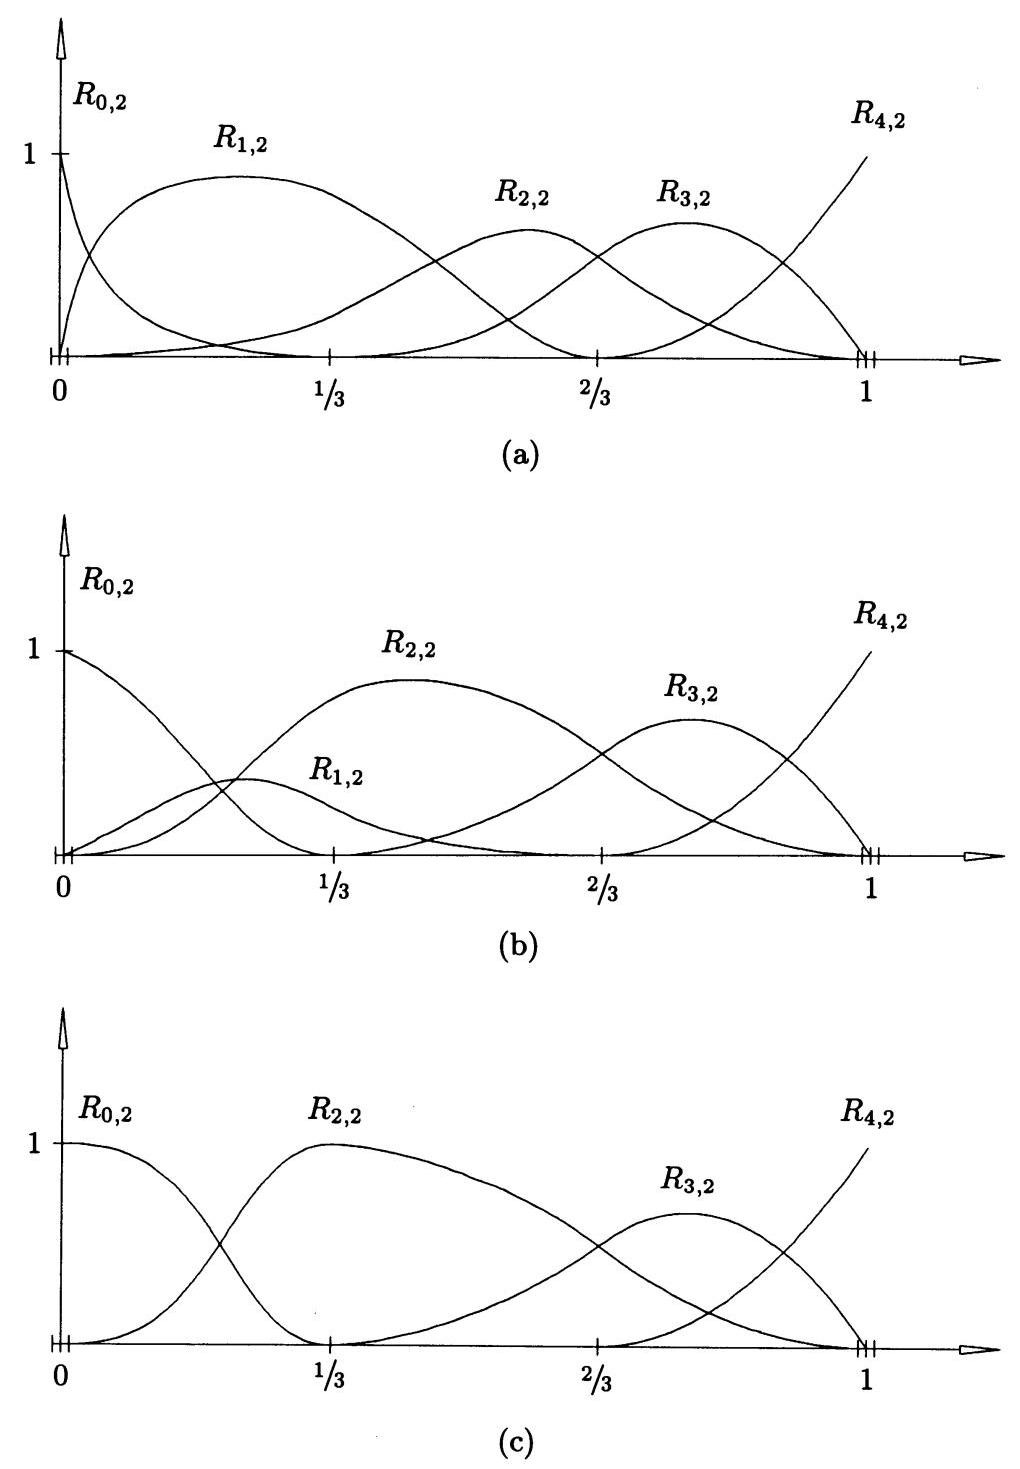
\includegraphics[max width=0.9\textwidth]{images/0193ba0d-ab19-7138-9798-cb281ce60de0_133_256_263_1020_1469_0.jpg}
\end{center}
\hspace*{3em} 

图 4.5. 图 4.4 曲线的二次基函数。(a) \({w}_{1} = 4\) ; (b) \({w}_{1} = 3/{10}\) ; (c) \({w}_{1} = 0\) 。

因此

\[
{\mathbf{C}}^{w}\left( 1\right)  = \frac{1}{2}{\mathbf{P}}_{1}^{w} + \frac{1}{2}{\mathbf{P}}_{2}^{w} = \frac{1}{2}\left( {4,4,4}\right)  + \frac{1}{2}\left( {3,2,1}\right)  = \left( {\frac{7}{2},3,\frac{5}{2}}\right)
\]

124 有理 B 样条曲线和曲面

\begin{center}
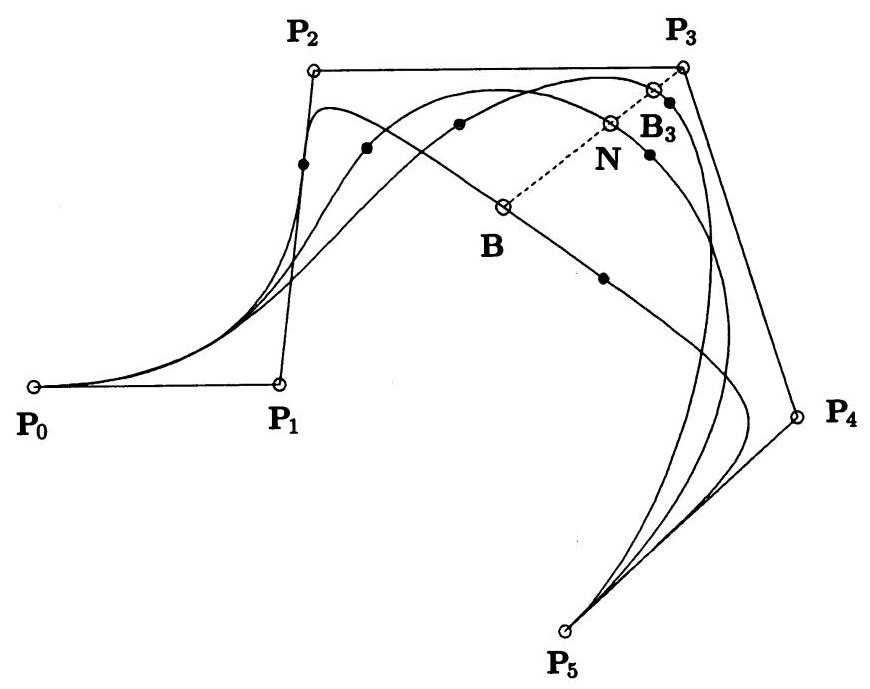
\includegraphics[max width=0.7\textwidth]{images/0193ba0d-ab19-7138-9798-cb281ce60de0_134_329_259_870_689_0.jpg}
\end{center}
\hspace*{3em} 

图 4.6. 权重 \({w}_{3}\) 的修改。

投影产生

\[
\mathbf{C}\left( 1\right)  = \left( {\frac{7}{5},\frac{6}{5}}\right)
\]

算法 A4.1 计算在固定 \(u\) 值下的有理 B-样条曲线上的点。它基于公式 (4.5)，即假设数组 \(\mathrm{{Pw}}\) 中的加权控制点(本书其余部分的所有算法均如此，除非另有说明)。因此，Pw[i] 包含 \({\mathbf{P}}_{i} = \left( {{w}_{i}{x}_{i},{w}_{i}{y}_{i},{w}_{i}{z}_{i},{w}_{i}}\right)\) 。Cw 表示 \({\mathbf{C}}^{w}\left( u\right)\) 上的四维点，而 \(\mathbf{C}\) 表示 \(\mathbf{C}\left( u\right)\) 上的三维点(输出)。在本书的其余部分，我们使用符号 \(C = {Cw}/w\) 来表示投影。

\HRule

ALGORITHM A4.1

\hspace*{1em} CurvePoint(n, p, U, Pw, u, C)

\hspace*{2em} \{ /* Compute point on rational B-spline curve */

\hspace*{3em} /* Input: n, p, U, Pw, u */

\hspace*{3em} /* Output: C */

\hspace*{2em} span \(= \operatorname{FindSpan}\left( {\mathrm{n},\mathrm{p},\mathrm{u},\mathrm{U}}\right)\) ;

\hspace*{2em} BasisFuns(span, u, p, U, N);

\hspace*{2em} Cw = 0.0 ;

\hspace*{2em} for (j=0; j<=p; j++)

\hspace*{3em} \(\mathrm{{Cw}} = \mathrm{{Cw}} + \mathrm{N}\left\lbrack  \mathrm{j}\right\rbrack   * \mathrm{{Pw}}\left\lbrack  {\mathrm{{span}} - \mathrm{p} + \mathrm{j}}\right\rbrack  ;\)

\hspace*{2em} \(\mathrm{C} = \mathrm{{Cw}}/\mathrm{w};\;/ *\) Divide by weight */

\hspace*{2em} \}

\HRule



\section{NURBS曲线的导数}

有理函数的导数是复杂的，涉及高次幂的分母。在第 3.3 节中，我们开发了计算非有理 B-样条曲线导数的公式和算法。这些公式和算法当然适用于 \({\mathbf{C}}^{w}\left( u\right)\) ，因为它是四维空间中的非有理曲线。在本节中，我们开发了公式，以导数 \(\mathbf{C}\left( u\right)\) 表达为 \({\mathbf{C}}^{w}\left( u\right)\) 的导数。

设

\[
\mathbf{C}\left( u\right)  = \frac{w\left( u\right) \mathbf{C}\left( u\right) }{w\left( u\right) } = \frac{\mathbf{A}\left( u\right) }{w\left( u\right) }
\]

其中 \(\mathbf{A}\left( u\right)\) 是向量值函数，其坐标是 \({\mathbf{C}}^{w}\left( u\right) \left( {\mathbf{A}\left( u\right) \text{ is the numerator of Eq. [4.1]). Then }}\right)\) 的前三个坐标

\[
{\mathbf{C}}^{\prime }\left( u\right)  = \frac{w\left( u\right) {\mathbf{A}}^{\prime }\left( u\right)  - {w}^{\prime }\left( u\right) \mathbf{A}\left( u\right) }{w{\left( u\right) }^{2}}
\]

\[
= \frac{w\left( u\right) {\mathbf{A}}^{\prime }\left( u\right)  - {w}^{\prime }\left( u\right) w\left( u\right) \mathbf{C}\left( u\right) }{w{\left( u\right) }^{2}} = \frac{{\mathbf{A}}^{\prime }\left( u\right)  - {w}^{\prime }\left( u\right) \mathbf{C}\left( u\right) }{w\left( u\right) } \tag{4.7}
\]

由于 \(\mathbf{A}\left( u\right)\) 和 \(w\left( u\right)\) 表示 \({\mathbf{C}}^{w}\left( u\right)\) 的坐标，我们使用公式 (3.4)-(3.6) 获得它们的第一导数。我们通过使用莱布尼茨法则对 \(\mathbf{A}\left( u\right)\) 进行求导来计算高阶导数

\[
{\mathbf{A}}^{\left( k\right) }\left( u\right)  = {\left( w\left( u\right) \mathbf{C}\left( u\right) \right) }^{\left( k\right) } = \mathop{\sum }\limits_{{i = 0}}^{k}\left( \begin{matrix} k \\  i \end{matrix}\right) {w}^{\left( i\right) }\left( u\right) {\mathbf{C}}^{\left( k - i\right) }\left( u\right)
\]

\[
= w\left( u\right) {\mathbf{C}}^{\left( k\right) }\left( u\right)  + \mathop{\sum }\limits_{{i = 1}}^{k}\left( \begin{matrix} k \\  i \end{matrix}\right) {w}^{\left( i\right) }\left( u\right) {\mathbf{C}}^{\left( k - i\right) }\left( u\right)
\]

从中我们得到

\[
{\mathbf{C}}^{\left( k\right) }\left( u\right)  = \frac{{\mathbf{A}}^{\left( k\right) }\left( u\right)  - \mathop{\sum }\limits_{{i = 1}}^{k}\left( \begin{matrix} k \\  i \end{matrix}\right) {w}^{\left( i\right) }\left( u\right) {\mathbf{C}}^{\left( k - i\right) }\left( u\right) }{w\left( u\right) } \tag{4.8}
\]

方程 (4.8) 给出了 \(k\) 的 \(\mathbf{C}\left( u\right)\) 次导数，以 \(k\) 的 \(\mathbf{A}\left( u\right)\) 次导数以及 \(\mathbf{C}\left( u\right)\) 和 \(w\left( u\right)\) 的第一到 (k - 1) 次导数为基础。导数 \({\mathbf{A}}^{\left( k\right) }\left( u\right)\) 和 \({w}^{\left( i\right) }\left( u\right)\) 是通过使用方程 (3.3) 和算法 A3.2 或方程 (3.8) 和算法 A3.4 获得的。

让我们推导 NURBS 曲线在其端点 \(\left( {u = 0,u = 1}\right)\) 的第一导数的表达式。从方程 (3.7) 我们得到

\[
{\mathbf{A}}^{\prime }\left( 0\right)  = \frac{p}{{u}_{p + 1}}\left( {{w}_{1}{\mathbf{P}}_{1} - {w}_{0}{\mathbf{P}}_{0}}\right) \;{w}^{\prime }\left( 0\right)  = \frac{p}{{u}_{p + 1}}\left( {{w}_{1} - {w}_{0}}\right)
\]

并且从方程 (4.7)

\[
{\mathbf{C}}^{\prime }\left( 0\right)  = \frac{\frac{p}{{u}_{p + 1}}\left( {{w}_{1}{\mathbf{P}}_{1} - {w}_{0}{\mathbf{P}}_{0}}\right)  - \frac{p}{{u}_{p + 1}}\left( {{w}_{1} - {w}_{0}}\right) {\mathbf{P}}_{0}}{{w}_{0}}
\]

从中可以得出

\[
{\mathbf{C}}^{\prime }\left( 0\right)  = \frac{p}{{u}_{p + 1}}\frac{{w}_{1}}{{w}_{0}}\left( {{\mathbf{P}}_{1} - {\mathbf{P}}_{0}}\right)  \tag{4.9}
\]

类似地

\[
{\mathbf{C}}^{\prime }\left( 1\right)  = \frac{p}{1 - {u}_{m - p - 1}}\frac{{w}_{n - 1}}{{w}_{n}}\left( {{\mathbf{P}}_{n} - {\mathbf{P}}_{n - 1}}\right)  \tag{4.10}
\]

\section*{示例}

Ex4.2 考虑在第 1.4 节中给出的二次有理贝塞尔圆弧(图 1.19b)。这是一个在节点向量 \(U = \{ 0,0,0\) ， \(1,1,1\}\) 上的 NURBS 曲线，具有 \(\left\{  {\mathbf{P}}_{i}\right\}   = \{ \left( {1,0}\right) ,\left( {1,1}\right) ,\left( {0,1}\right) \}\) 和 \(\left\{  {w}_{i}\right\}   = \{ 1,1,2\}\) 。从方程 (4.9) 和 (4.10) 我们得到

\[
{\mathbf{C}}^{\prime }\left( 0\right)  = \frac{2}{1}\frac{1}{1}\left( {{\mathbf{P}}_{1} - {\mathbf{P}}_{0}}\right)  = \left( {0,2}\right)
\]

\[
{\mathbf{C}}^{\prime }\left( 1\right)  = \frac{2}{1 - 0}\frac{1}{2}\left( {{\mathbf{P}}_{2} - {\mathbf{P}}_{1}}\right)  = \left( {-1,0}\right)
\]

从方程 (4.8)

\[
{\mathbf{C}}^{\prime \prime }\left( 0\right)  = \frac{{\mathbf{A}}^{\prime \prime }\left( 0\right)  - 2{w}^{\prime }\left( 0\right) {\mathbf{C}}^{\prime }\left( 0\right)  - {w}^{\prime \prime }\left( 0\right) \mathbf{C}\left( 0\right) }{{w}_{0}}
\]

从方程 (3.9) 或方程 (1.10)

\[
{\mathbf{A}}^{\prime \prime }\left( 0\right)  = 2\left( {{w}_{0}{\mathbf{P}}_{0} - 2{w}_{1}{\mathbf{P}}_{1} + {w}_{2}{\mathbf{P}}_{2}}\right)
\]

并且

\[
{w}^{\prime \prime }\left( 0\right)  = 2\left( {{w}_{0} - 2{w}_{1} + {w}_{2}}\right)
\]

从 \({w}^{\prime }\left( 0\right)  = 2\left( {{w}_{1} - {w}_{0}}\right)\) 可以得出

\[
{\mathbf{C}}^{\prime \prime }\left( 0\right)  = \frac{2}{{w}_{0}}\left\lbrack  {{w}_{0}{\mathbf{P}}_{0} - 2{w}_{1}{\mathbf{P}}_{1} + {w}_{2}{\mathbf{P}}_{2} - 4\left( {{w}_{1} - {w}_{0}}\right) \left( {{\mathbf{P}}_{1} - {\mathbf{P}}_{0}}\right) }\right.
\]

\[
\left. {-\left( {{w}_{0} - 2{w}_{1} + {w}_{2}}\right) {\mathbf{P}}_{0}}\right\rbrack
\]

\[
= 2\left( {{\mathbf{P}}_{0} - 2{\mathbf{P}}_{1} + 2{\mathbf{P}}_{2} - {\mathbf{P}}_{0}}\right)  = 4\left( {{\mathbf{P}}_{2} - {\mathbf{P}}_{1}}\right)  = \left( {-4,0}\right)
\]

\({\mathbf{C}}^{\prime \prime }\left( 1\right)\) 的计算留作练习。

现在假设 \(u\) 是固定的，并且 \(\mathbf{A}\left( u\right)\) 和 \(w\left( u\right)\) 的零阶到 \(d\) 阶导数已经计算并分别加载到数组 Aders 和 wders 中，即 \({\mathbf{C}}^{w}\left( u\right)\) 已经被求导，其坐标分离到 Aders 和 wders 中。算法 A4.2 计算点 \(\mathbf{C}\left( u\right)\) 和导数 \({\mathbf{C}}^{\left( k\right) }\left( u\right) ,1 \leq  k \leq  d\) 。曲线点返回在 \(\mathrm{{CK}}\left\lbrack  0\right\rbrack\) 中，第 \(k\) 阶导数返回在 CK[k] 中。数组 Bin[][] 包含预计算的二项式系数(Bin \(\left\lbrack  \mathrm{k}\right\rbrack  \left\lbrack  \mathrm{i}\right\rbrack\) 是 \(\left( \begin{array}{l} k \\  i \end{array}\right)\) )。

\HRule

ALGORITHM A4.2

\hspace*{1em} RatCurveDerivs (Aders, wders, d, CK)

\hspace*{3em} \{ /* Compute C(u) derivatives from Cw(u) derivatives */

\hspace*{4em} /* Input: Aders, wders, d */

\hspace*{4em} /* Output: CK */

\hspace*{2em} for (k=0; k<=d; k++)

\hspace*{4em} \{

\hspace*{4em} v = Aders[k];

\hspace*{4em} for (i=1; i<=k; i++)

\hspace*{5em} v = v - Bin[k][i]*wders[i]*CK[k-i];

\hspace*{4em} CK[k] = v/wders[0];

\hspace*{4em} \}

\hspace*{2em} \}

\HRule

图 4.7 显示了三次 NURBS 曲线的一阶、二阶和三阶导数。导数向量分别缩放为 0.4、0.08 和 0.03。

\begin{center}
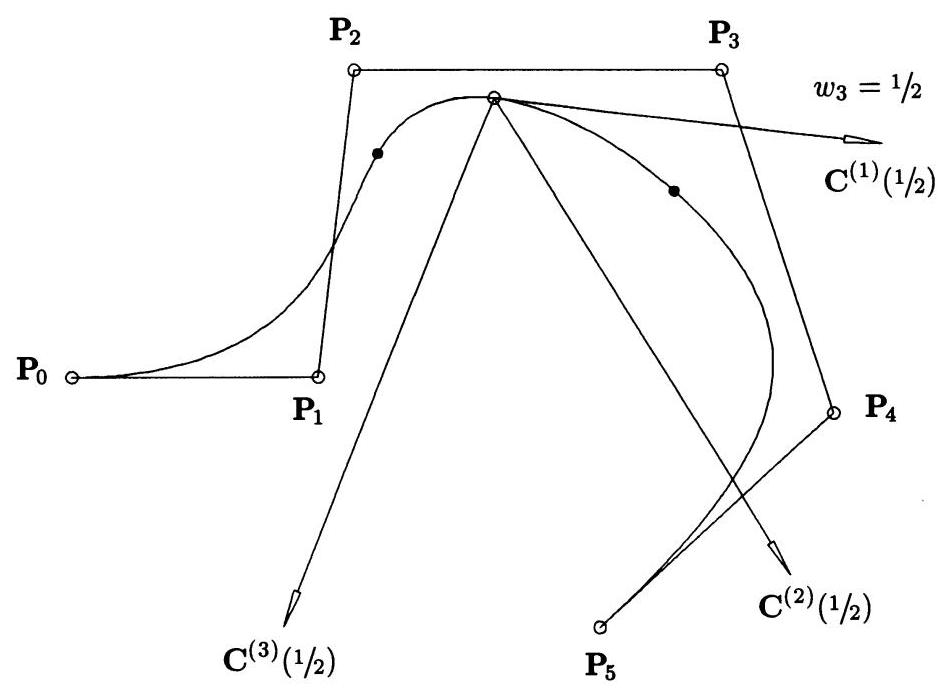
\includegraphics[max width=0.8\textwidth]{images/0193ba0d-ab19-7138-9798-cb281ce60de0_137_287_1340_947_693_0.jpg}
\end{center}
\hspace*{3em} 

图 4.7. 在 \(u = 1/2\) 处计算的三次 NURBS 曲线的一阶、二阶和三阶导数，使用 \({w}_{3} = 1/2\) 和 \({w}_{i} = 1,i \neq  3\) 。



\section{NURBS曲面的定义与性质}

在 \(u\) 方向上为 \(p\) 阶，在 \(v\) 方向上为 \(q\) 阶的 NURBS 曲面是一个双变量向量值分段有理函数，形式为

\[
\mathbf{S}\left( {u,v}\right)  = \frac{\mathop{\sum }\limits_{{i = 0}}^{n}\mathop{\sum }\limits_{{j = 0}}^{m}{N}_{i,p}\left( u\right) {N}_{j,q}\left( v\right) {w}_{i,j}{\mathbf{P}}_{i,j}}{\mathop{\sum }\limits_{{i = 0}}^{n}\mathop{\sum }\limits_{{j = 0}}^{m}{N}_{i,p}\left( u\right) {N}_{j,q}\left( v\right) {w}_{i,j}}\;0 \leq  u,v \leq  1 \tag{4.11}
\]

\(\left\{  {\mathbf{P}}_{i,j}\right\}\) 形成一个双向控制网， \(\left\{  {w}_{i,j}\right\}\) 是权重， \(\left\{  {{N}_{i,p}\left( u\right) }\right\}\) 和 \(\left\{  {{N}_{j,q}\left( v\right) }\right\}\) 是定义在节点向量上的非有理 B 样条基函数。

\[
U = \left\{  {\underset{p + 1}{\underbrace{0,\ldots ,0}},{u}_{p + 1},\ldots ,{u}_{r - p - 1},\underset{p + 1}{\underbrace{1,\ldots ,1}}}\right\}
\]

\[
V = \{ \underset{q + 1}{\underbrace{0,\ldots ,0}},{v}_{q + 1},\ldots ,{v}_{s - q - 1},\underset{q + 1}{\underbrace{1,\ldots ,1}}\}
\]

其中 \(r = n + p + 1\) 和 \(s = m + q + 1\) 。

引入分段有理基函数

\[
{R}_{i,j}\left( {u,v}\right)  = \frac{{N}_{i,p}\left( u\right) {N}_{j,q}\left( v\right) {w}_{i,j}}{\mathop{\sum }\limits_{{k = 0}}^{n}\mathop{\sum }\limits_{{l = 0}}^{m}{N}_{k,p}\left( u\right) {N}_{l,q}\left( v\right) {w}_{k,l}} \tag{4.12}
\]

表面方程 (4.11) 可以写成

\[
\mathbf{S}\left( {u,v}\right)  = \mathop{\sum }\limits_{{i = 0}}^{n}\mathop{\sum }\limits_{{j = 0}}^{m}{R}_{i,j}\left( {u,v}\right) {\mathbf{P}}_{i,j} \tag{4.13}
\]

图 4.8 和 4.9 显示了 NURBS 曲面的示例。

函数的主要属性 \({R}_{i,j}\left( {u,v}\right)\) 大致与第 3.4 节中给出的非理性基函数的属性相同 \({N}_{i,p}\left( u\right) {N}_{j,q}\left( v\right)\) 。我们在此总结它们。

P4.15 非负性: \({R}_{i,j}\left( {u,v}\right)  \geq  0\) 对所有 \(i,j,u\) 和 \(v\) 成立；

P4.16 单位划分: \(\mathop{\sum }\limits_{{i = 0}}^{n}\mathop{\sum }\limits_{{j = 0}}^{m}{R}_{i,j}\left( {u,v}\right)  = 1\) 对所有 \(\left( {u,v}\right)  \in  \left\lbrack  {0,1}\right\rbrack   \times  \left\lbrack  {0,1}\right\rbrack\) 成立；

P4.17 局部支持: \({R}_{i,j}\left( {u,v}\right)  = 0\) 如果 (u, v) 在由 \(\left\lbrack  {{u}_{i},{u}_{i + p + 1}}\right)  \times  \left\lbrack  {{v}_{j},{v}_{j + q + 1}}\right)\) 给出的矩形之外；

P4.18 在任何给定的形式为 \(\left\lbrack  {{u}_{{i}_{0}},{u}_{{i}_{0} + 1}}\right)  \times  \left\lbrack  {{v}_{{j}_{0}},{v}_{{j}_{0} + 1}}\right)\) 的矩形中，最多有 \(\left( {p + 1}\right) \left( {q + 1}\right)\) 个基函数非零，特别是 \({R}_{i,j}\left( {u,v}\right)\) 对于 \({i}_{0} - p \leq  i \leq  {i}_{0}\) 和 \({j}_{0} - q \leq  j \leq  {j}_{0}\) 是非零的；

P4.19 极值:如果 \(p > 0\) 和 \(q > 0\) ，则 \({R}_{i,j}\left( {u,v}\right)\) 恰好达到一个最大值；

\begin{center}
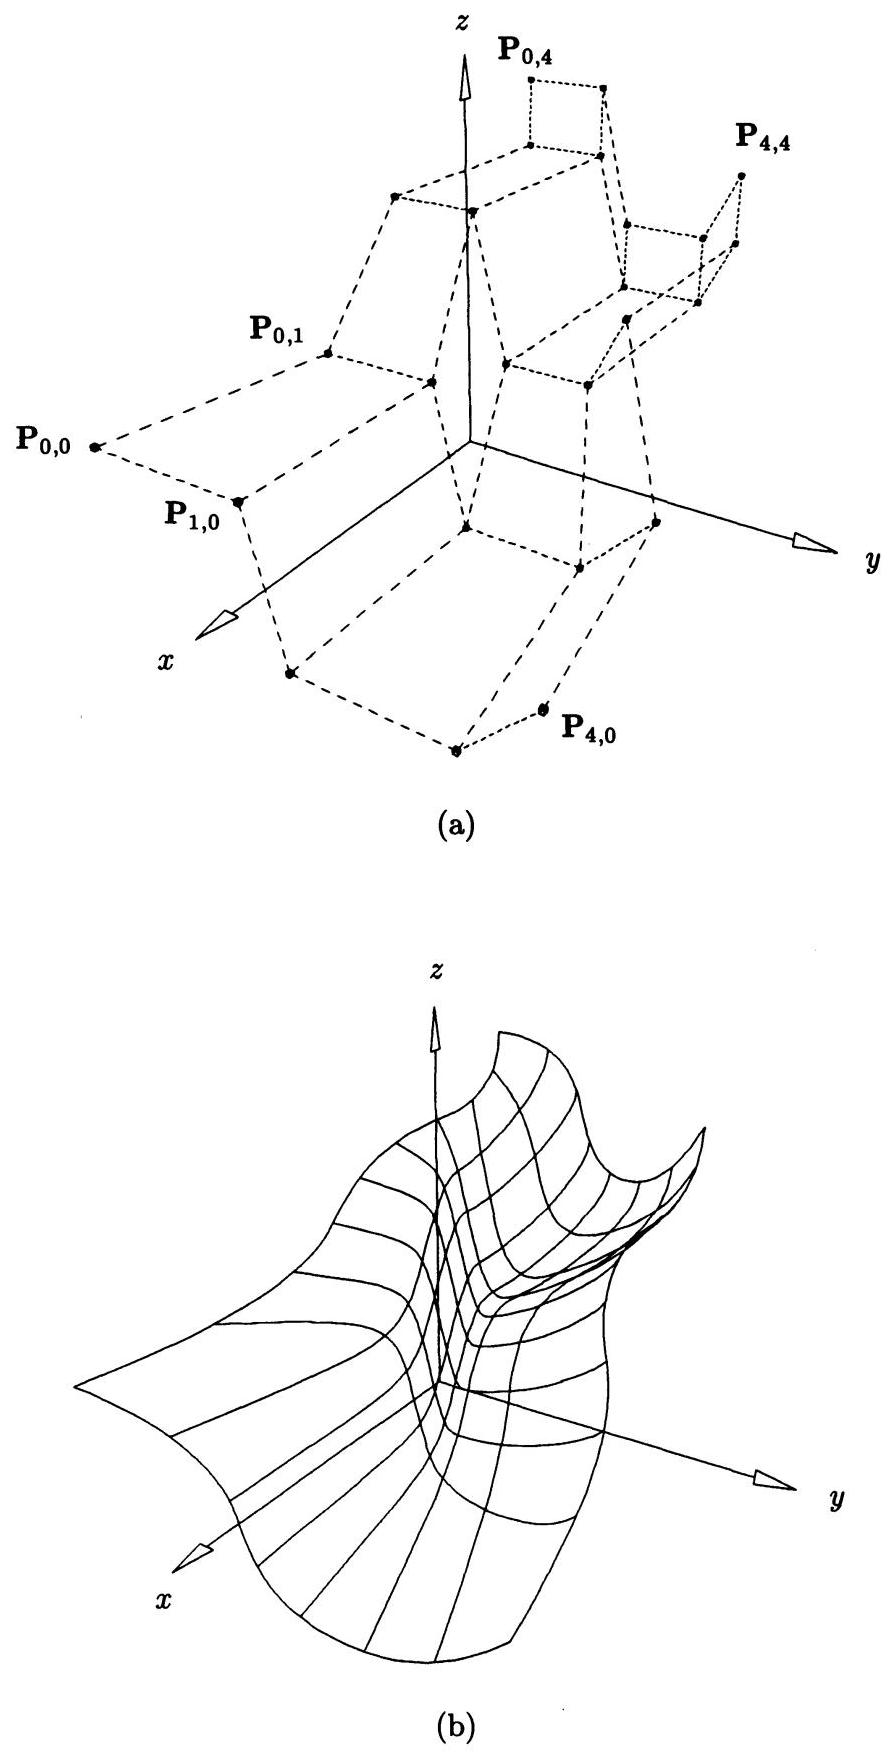
\includegraphics[max width=0.8\textwidth]{images/0193ba0d-ab19-7138-9798-cb281ce60de0_139_318_257_890_1758_0.jpg}
\end{center}
\hspace*{3em} 

图 4.8. 控制网和二次 NURBS 曲面， \({w}_{1,1} = {w}_{1,2} = {w}_{2,1} = {w}_{2,2} =\) 10，其他权重为 \(1.U = V = \{ 0,0,0,1/3,2/3,1,1,1\}\) 。(a) 控制网；(b) 二次 NURBS 曲面。

\begin{center}
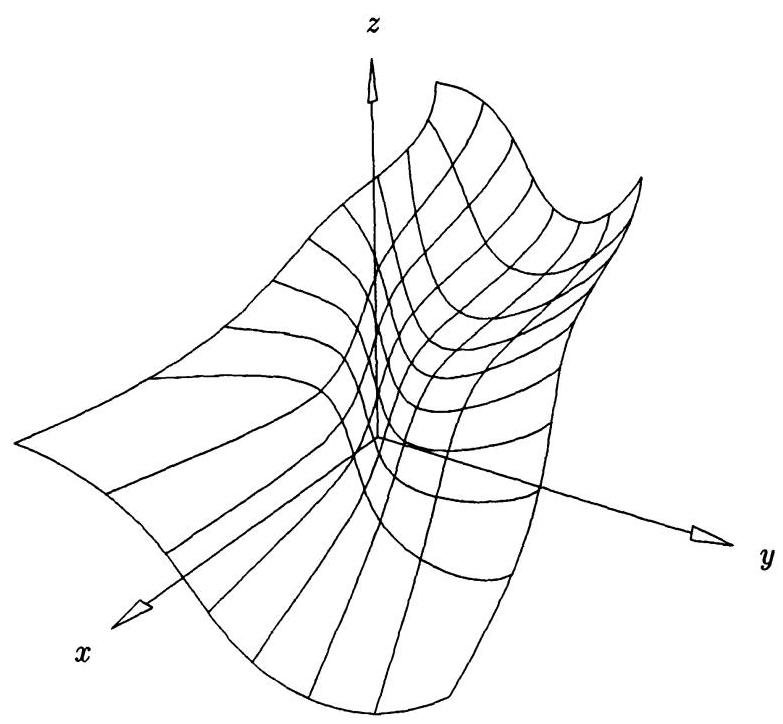
\includegraphics[max width=0.7\textwidth]{images/0193ba0d-ab19-7138-9798-cb281ce60de0_140_374_266_783_724_0.jpg}
\end{center}
\hspace*{3em} 

图 4.9. 由图 4.8a 中的控制网定义的三次 NURBS 曲面，权重与图 4.8 中相同。

P4. \({20}{R}_{0,0}\left( {0,0}\right)  = {R}_{n,0}\left( {1,0}\right)  = {R}_{0,m}\left( {0,1}\right)  = {R}_{n,m}\left( {1,1}\right)  = 1\) ;

P4.21 可微性:在由 \(u\) 和 \(v\) 节点线形成的矩形内部，所有 \({R}_{i,j}\left( {u,v}\right)\) 的偏导数存在。在 \(u\) 节点 (vknot) 处，它在 \(u\left( v\right)\) 方向上是 \(p - k\left( {q - k}\right)\) 次可微的，其中 \(k\) 是节点的重数；

P4.22 如果所有 \({w}_{i,j} = a\) 对于 \(0 \leq  i \leq  n,0 \leq  j \leq  m\) 和 \(a \neq  0\) 成立，则 \({R}_{i,j}\left( {u,v}\right)  =\)  \({N}_{i,p}\left( u\right) {N}_{j,q}\left( v\right)\) 对所有 \(i,j\) 成立。

性质 P4.15-P4.22 产生了 NURBS 曲面的以下重要几何性质:

P4.23 角点插值: \(\mathbf{S}\left( {0,0}\right)  = {\mathbf{P}}_{0,0},\mathbf{S}\left( {1,0}\right)  = {\mathbf{P}}_{n,0},\mathbf{S}\left( {0,1}\right)  =\)  \({\mathbf{P}}_{0,m}\) ，和 \(\mathbf{S}\left( {1,1}\right)  = {\mathbf{P}}_{n,m}\) ；

P4.24 仿射不变性:通过对控制点应用仿射变换来对曲面进行仿射变换；

P4.25 强凸包性质:假设 \({w}_{i,j} \geq  0\) 对所有 \(i,j\) 成立。如果 \(\left( {u,v}\right)  \in\)  \(\left\lbrack  {{u}_{{i}_{0}},{u}_{{i}_{0} + 1}}\right)  \times  \left\lbrack  {{v}_{{j}_{0}},{v}_{{j}_{0} + 1}}\right)\) ，则 \(\mathbf{S}\left( {u,v}\right)\) 在控制点 \({\mathbf{P}}_{i,j},{i}_{0} - p \leq  i \leq  {i}_{0}\) 和 \({j}_{0} - q \leq  j \leq  {j}_{0}\) 的凸包内；

P4.26 局部修改:如果 \({\mathbf{P}}_{i,j}\) 被移动，或者 \({w}_{i,j}\) 被改变，它只会影响矩形 \(\left\lbrack  {{u}_{i},{u}_{i + p + 1}}\right)  \times  \left\lbrack  {{v}_{j},{v}_{j + q + 1}}\right)\) 内的曲面形状；

P4.27 非理性 B-spline 和 Bézier 以及理性 Bézier 曲面是 NURBS 曲面的特例；

P4.28 可微性: \(\mathbf{S}\left( {u,v}\right)\) 在一个重数为 \(k\) 的 \(u\) 节点 (vknot) 处对 \(u\left( v\right)\) 是 \(p - k\left( {q - k}\right)\) 次可微的。

我们注意到，目前尚无已知的 NURBS 曲面的变差减小性质(见 [Prau92])。

我们可以使用控制点移动和权重修改来局部改变 NURBS 曲面的形状。图 4.10 和 4.11 显示了当单个权重 \({w}_{i,j}\) 被修改时，对基函数 \({R}_{i,j}\left( {u,v}\right)\) 和曲面形状的影响。将这些图与图 3.19b 和 3.20a, b 进行比较。从定性上看，对曲面的影响是:假设 \(\left( {u,v}\right)  \in  \left\lbrack  {{u}_{i},{u}_{i + p + 1}}\right)  \times  \left\lbrack  {{v}_{j},{v}_{j + q + 1}}\right)\) ；那么如果 \({w}_{i,j}\) 增加(减少)，点 \(\mathbf{S}\left( {u,v}\right)\) 将更靠近(远离) \({\mathbf{P}}_{i,j}\) ，因此曲面被拉向(推离) \({\mathbf{P}}_{i,j}\) 。与曲线的情况一样， \(\mathbf{S}\left( {u,v}\right)\) 的移动是沿着一条直线。在图 \({4.12}\left( {u,v}\right)\) 中， \({w}_{2,2}\) 是变化的。

\[
\mathbf{S} = \mathbf{S}\left( {u,v;{w}_{2,2} = 0}\right)
\]

\[
\mathbf{M} = \mathbf{S}\left( {u,v;{w}_{2,2} = 1}\right)  \tag{4.14}
\]

然后由 \(\mathbf{S}\) 和 \(\mathbf{M}\) 定义的直线通过 \({\mathbf{P}}_{2,2}\) ，对于任意的 \({w}_{2,2},0 < {w}_{2,2} < \infty ,{\mathbf{S}}_{2,2} = \mathbf{S}\left( {u,v;{w}_{2,2}}\right)\) ，它位于这条线段 \(\mathbf{S}\) 和 \({\mathbf{P}}_{2,2}\) 之间。

\begin{center}
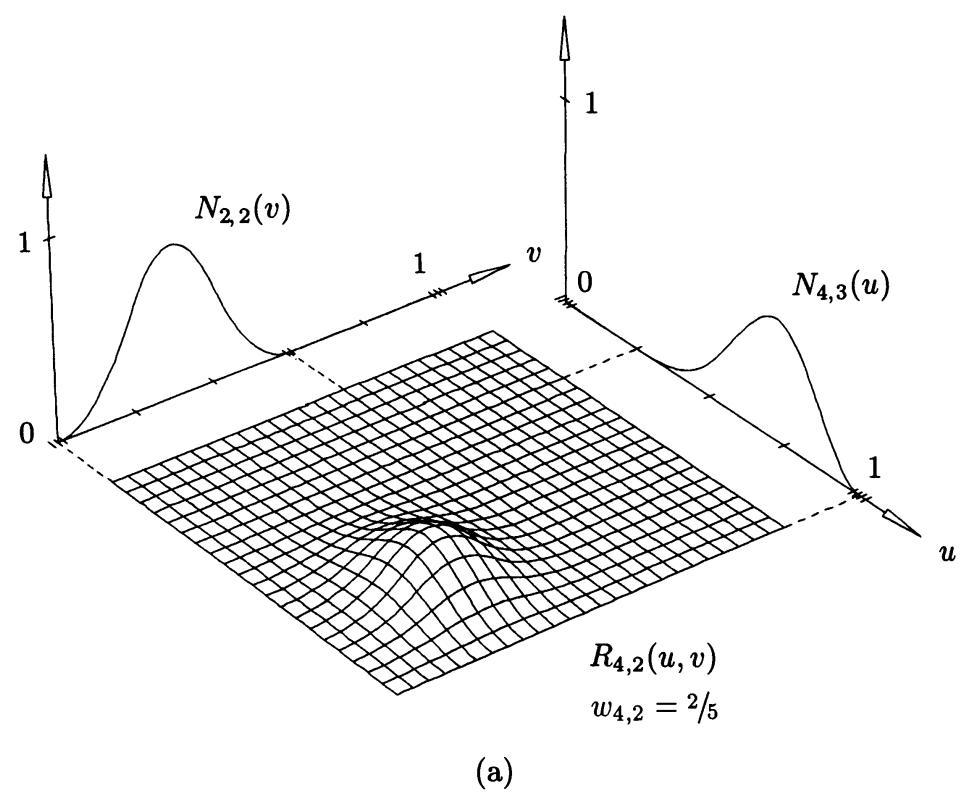
\includegraphics[max width=0.8\textwidth]{images/0193ba0d-ab19-7138-9798-cb281ce60de0_141_280_1216_968_799_0.jpg}
\end{center}
\hspace*{3em} 

图 4.10. 基函数 \({R}_{4,2,\left( {u,v}\right) }\) ，对于所有 \(\left( {i,j}\right)  \neq  \left( {4,2}\right) .\left( a\right) {w}_{4,2} = 2/5;\) 的 \(U = \{ 0,0,0,0,1/4,1/2,3/4,1,1,1\}\) 和 \(V = \{ 0,0,0,1/5,2/5,3/5,3/5,4/5,1,1/1\} .{w}_{i,j} = 1\) (b) \({w}_{4,2} = 6\) 。

\begin{center}
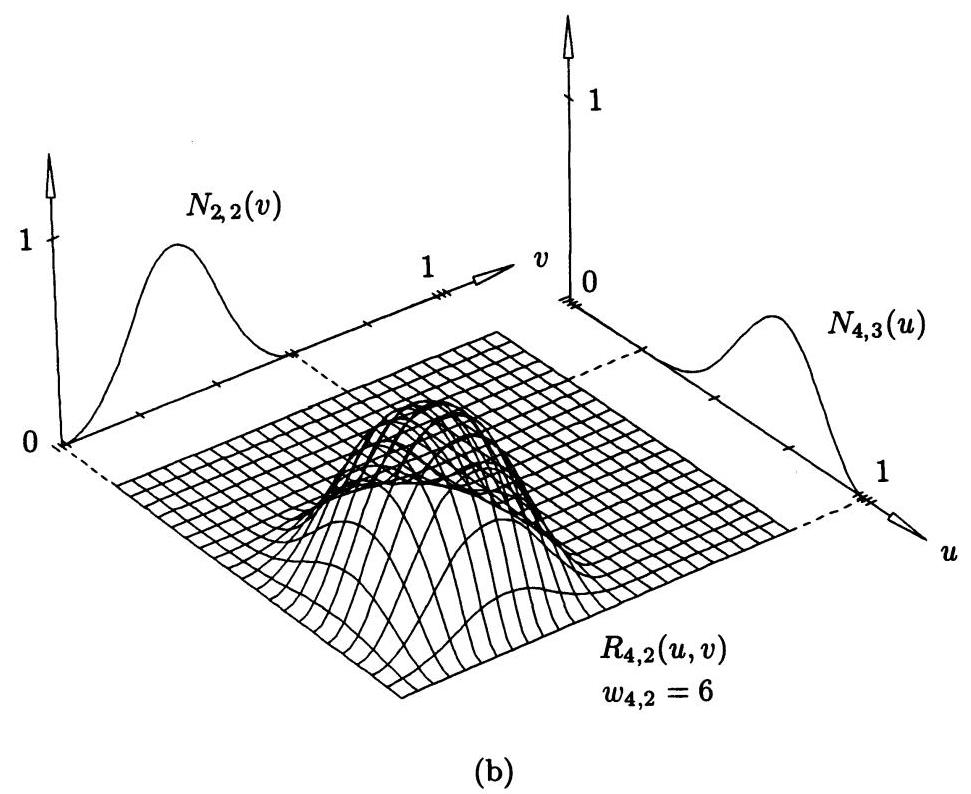
\includegraphics[max width=0.8\textwidth]{images/0193ba0d-ab19-7138-9798-cb281ce60de0_142_281_262_971_794_0.jpg}
\end{center}
\hspace*{3em} 

图 4.10. (续)

使用齐次坐标表示 NURBS 曲面是方便的，

即

\[
{\mathbf{S}}^{w}\left( {u,v}\right)  = \mathop{\sum }\limits_{{i = 0}}^{n}\mathop{\sum }\limits_{{j = 0}}^{m}{N}_{i,p}\left( u\right) {N}_{j,q}\left( v\right) {\mathbf{P}}_{i,j}^{w} \tag{4.15}
\]

其中 \({\mathbf{P}}_{i,j}^{w} = \left( {{w}_{i,j}{x}_{i,j},{w}_{i,j}{y}_{i,j},{w}_{i,j}{z}_{i,j},{w}_{i,j}}\right)\) 。然后 \(\mathbf{S}\left( {u,v}\right)  = H\left\{  {{\mathbf{S}}^{w}\left( {u,v}\right) }\right\}\) 。我们可以交替地将 \({\mathbf{S}}^{w}\left( {u,v}\right)\) 或 \(\mathbf{S}\left( {u,v}\right)\) 称为 NURBS 曲面。严格来说， \({\mathbf{S}}^{w}\left( {u,v}\right)\) 是一个张量积的分段多项式曲面，位于四维空间中。 \(\mathbf{S}\left( {u,v}\right)\) 是一个分段有理曲面，位于三维空间中；它不是一个张量积曲面，因为 \({R}_{i,j}\left( {u,v}\right)\) 不是单变量基函数的乘积。

\section*{示例}

Ex4.3 设 \({\mathbf{S}}^{w}\left( {u,v}\right)  = \mathop{\sum }\limits_{{i = 0}}^{7}\mathop{\sum }\limits_{{j = 0}}^{4}{N}_{i,2}\left( u\right) {N}_{j,2}\left( v\right)\) ，具有

\[
U = \{ 0,0,0,1,2,3,4,4,5,5,5\}
\]

和

\[
V = \{ 0,0,0,1,2,3,3,3\}
\]

让我们在 \(\left( {u,v}\right)  = \left( {5/2,1}\right)\) 处评估表面。然后 \(u \in  \left\lbrack  {{u}_{4},{u}_{5}}\right)\) 和 \(v \in  \left\lbrack  {{v}_{3},{v}_{4}}\right)\) ，根据第 3.2 节和第 4.2 节，我们知道

\[
{N}_{2,2}\left( \frac{5}{2}\right)  = \frac{1}{8}\;{N}_{3,2}\left( \frac{5}{2}\right)  = \frac{6}{8}\;{N}_{4,2}\left( \frac{5}{2}\right)  = \frac{1}{8}
\]

\begin{center}
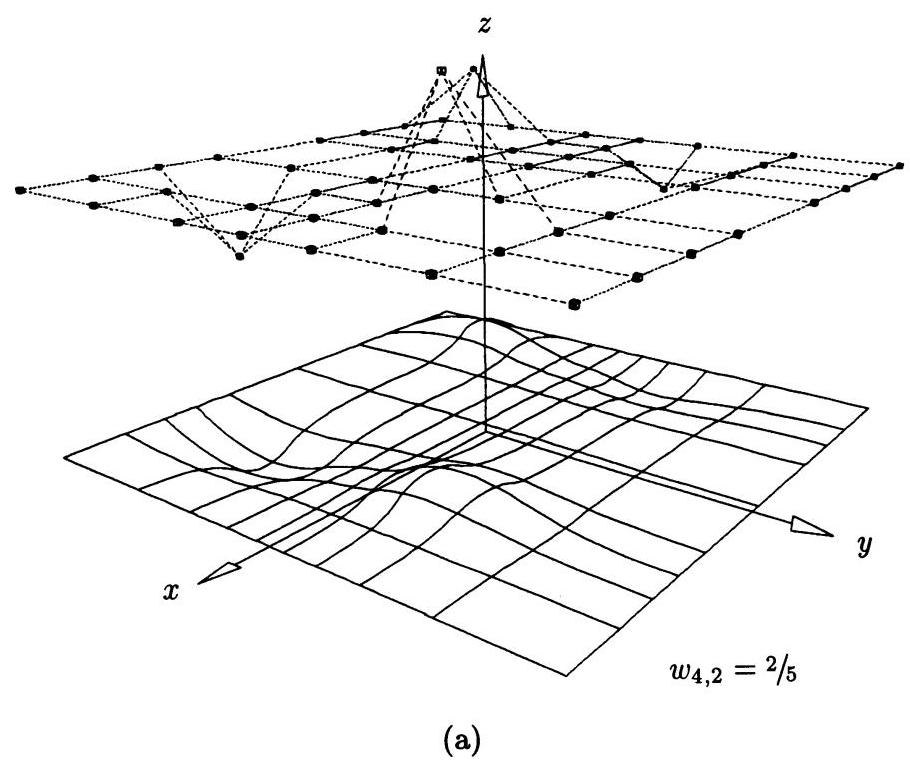
\includegraphics[max width=0.8\textwidth]{images/0193ba0d-ab19-7138-9798-cb281ce60de0_143_313_250_910_763_0.jpg}
\end{center}
\hspace*{3em} 

图 4.11。与图 4.10 对应的立方 \(\times\) 二次曲面，控制网格偏移以便更好地可视化。(a) \({w}_{4,2} = 2/5\) ；(b) \({w}_{4,2} = 6\) 。

和

\[
{N}_{1,2}\left( 1\right)  = \frac{1}{2}\;{N}_{2,2}\left( 1\right)  = \frac{1}{2}\;{N}_{3,2}\left( 1\right)  = 0
\]

现在假设

\[
\left\lbrack  {\mathbf{P}}_{i,j}^{w}\right\rbrack   = \left\lbrack  \begin{array}{lll} \left( {0,2,4,1}\right) & \left( {0,6,4,2}\right) & \left( {0,2,0,1}\right) \\  \left( {4,6,8,2}\right) & \left( {{12},{24},{12},6}\right) & \left( {4,6,0,2}\right) \\  \left( {4,2,4,1}\right) & \left( {8,6,4,2}\right) & \left( {4,2,0,1}\right)  \end{array}\right\rbrack
\]

\[
i = 2,3,4;\;j = 1,2,3
\]

然后

\[
{\mathbf{S}}^{w}\left( {\frac{5}{2},1}\right)  = \left\lbrack  \begin{array}{lll} \frac{1}{8} & \frac{6}{8} & \frac{1}{8} \end{array}\right\rbrack   \times
\]

\[
\left\lbrack  \begin{matrix} \left( {0,2,4,1}\right) & \left( {0,6,4,2}\right) & \left( {0,2,0,1}\right) \\  \left( {4,6,8,2}\right) & \left( {{12},{24},{12},6}\right) & \left( {4,6,0,2}\right) \\  \left( {4,2,4,1}\right) & \left( {8,6,4,2}\right) & \left( {4,2,0,1}\right)  \end{matrix}\right\rbrack  \left\lbrack  \begin{matrix} \frac{1}{2} \\  \frac{1}{2} \\  0 \end{matrix}\right\rbrack
\]

\[
= \left( {\frac{54}{8},\frac{98}{8},\frac{68}{8},\frac{27}{8}}\right)
\]

投影得到

\[
\mathbf{S}\left( {\frac{5}{2},1}\right)  = \left( {2,\frac{98}{27},\frac{68}{27}}\right)
\]

\begin{center}
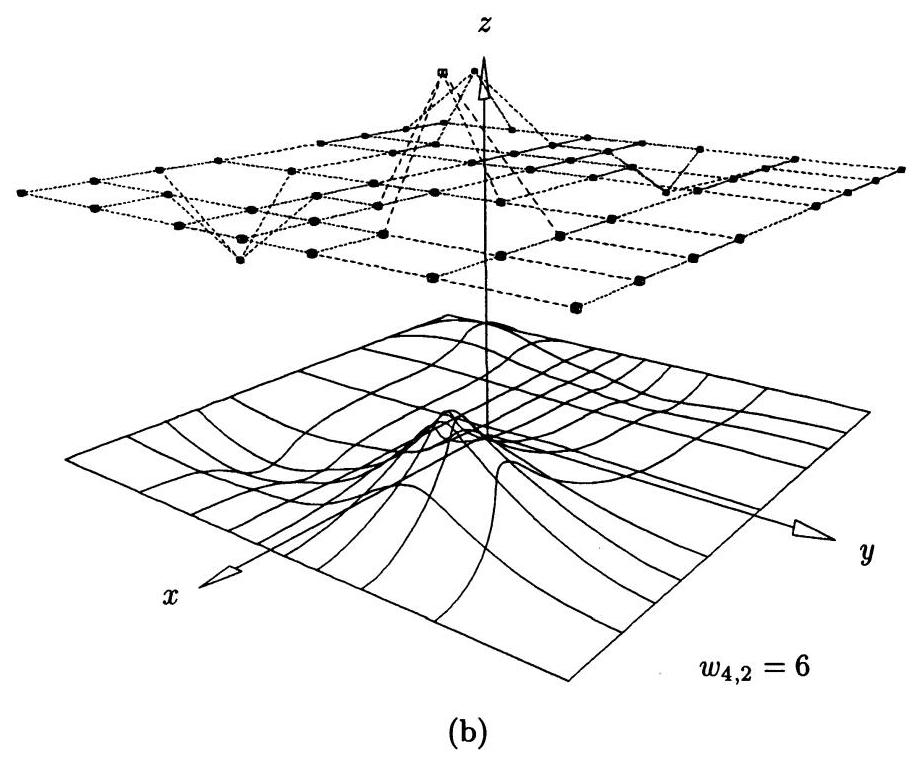
\includegraphics[max width=0.8\textwidth]{images/0193ba0d-ab19-7138-9798-cb281ce60de0_144_308_250_915_757_0.jpg}
\end{center}
\hspace*{3em} 

图 4.11。(续)

算法 A3.5 可以通过简单地允许数组 \(P\) 包含加权控制点(使用 Pw)，累积四维表面点在 \({Sw}\) 中，并在算法末尾插入行 \(S = {Sw}/w\) 来计算有理 B 样条曲面上的一个点。

\HRule

ALGORITHM A4.3

\hspace*{1em} SurfacePoint(n, p, U, m, q, V, Pw, u, v, S)

\hspace*{3em} \{ /* Compute point on rational B-spline surface */

\hspace*{4em} /* Input: n, p, U, m, q, V, Pw, u, v */

\hspace*{4em} /* Output: S */

\hspace*{3em} uspan = FindSpan(n, p, u, U);

\hspace*{3em} BasisFuns(uspan, u, p, U, Nu);

\hspace*{3em} vspan = FindSpan(m, q, v, V);

\hspace*{3em} BasisFuns(vspan, v, q, V, Nv);

\hspace*{3em} for (l=0; l<=q; l++)

\hspace*{4em} \{

\hspace*{4em} temp[1] = 0.0 ;

\hspace*{4em} for \(\left( {k = 0;k <  = p;k +  + }\right)\)

\hspace*{5em} temp[1] = temp[1] + Nu[k]*Pw[uspan-p+k][vspan-q+1];

\hspace*{4em} \}

\hspace*{3em} Sw = 0.0 ;

\hspace*{3em} for (l=0; l<=q; l++)

\hspace*{4em} Sw = Sw + Nv[1]*temp[1];

\hspace*{3em} \(S = {Sw}/w\)

\hspace*{3em} \}

\HRule

\begin{center}
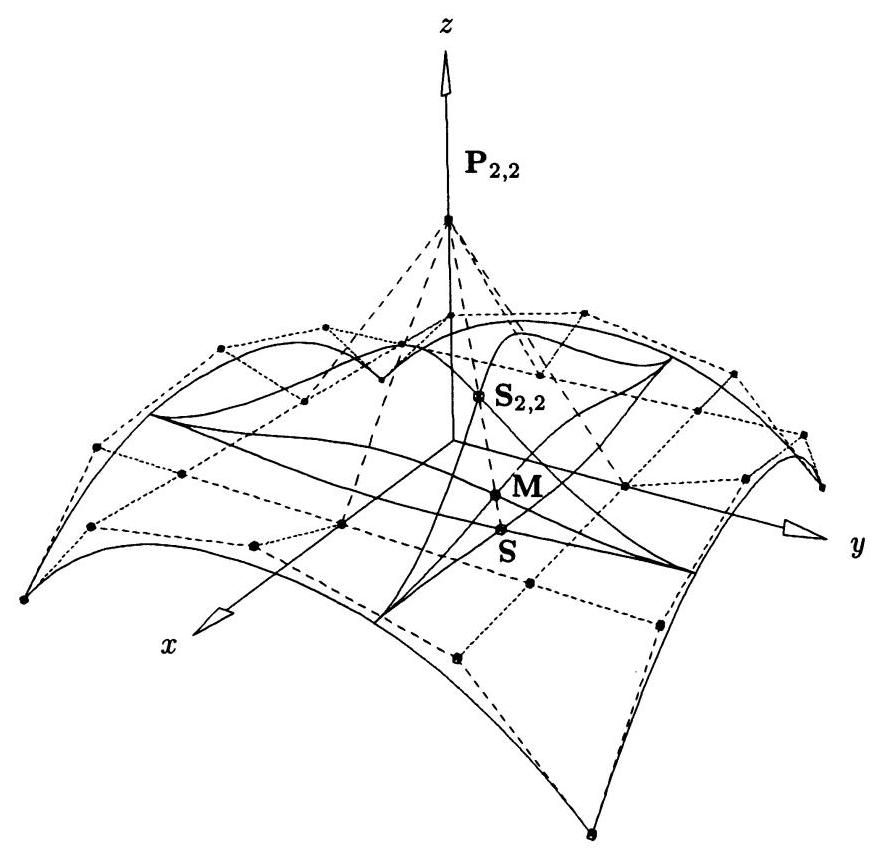
\includegraphics[max width=0.8\textwidth]{images/0193ba0d-ab19-7138-9798-cb281ce60de0_145_330_249_880_852_0.jpg}
\end{center}
\hspace*{3em} 

图 4.12。权重 \({w}_{2,2}\) 的修改。

通过应用方程 (3.14) 和 (3.15)，我们在 NURBS 表面上获得等参数曲线。首先，固定 \(u = {u}_{0}\)

\[
{\mathbf{C}}_{{u}_{0}}^{w}\left( v\right)  = {\mathbf{S}}^{w}\left( {{u}_{0},v}\right)  = \mathop{\sum }\limits_{{i = 0}}^{n}\mathop{\sum }\limits_{{j = 0}}^{m}{N}_{i,p}\left( {u}_{0}\right) {N}_{j,q}\left( v\right) {\mathbf{P}}_{i,j}^{w} \tag{4.16}
\]

\[
= \mathop{\sum }\limits_{{j = 0}}^{m}{N}_{j,q}\left( v\right) \left( {\mathop{\sum }\limits_{{i = 0}}^{n}{N}_{i,p}\left( {u}_{0}\right) {\mathbf{P}}_{i,j}^{w}}\right)
\]

\[
= \mathop{\sum }\limits_{{j = 0}}^{m}{N}_{j,q}\left( v\right) {\mathbf{Q}}_{j}^{w}\left( {u}_{0}\right)
\]

其中

\[
{\mathbf{Q}}_{j}^{w}\left( {u}_{0}\right)  = \mathop{\sum }\limits_{{i = 0}}^{n}{N}_{i,p}\left( {u}_{0}\right) {\mathbf{P}}_{i,j}^{w}
\]

类似地

\[
{\mathbf{C}}_{{v}_{0}}^{w}\left( u\right)  = \mathop{\sum }\limits_{{i = 0}}^{n}{N}_{i,p}\left( u\right) {\mathbf{Q}}_{i}^{w}\left( {v}_{0}\right)  \tag{4.17}
\]

在哪里

\[
{\mathbf{Q}}_{i}^{w}\left( {v}_{0}\right)  = \mathop{\sum }\limits_{{j = 0}}^{m}{N}_{j,q}\left( {v}_{0}\right) {\mathbf{P}}_{i,j}^{w}
\]

\({\mathbf{C}}_{{u}_{0}}^{w}\left( v\right) \left( {{\mathbf{C}}_{{v}_{0}}^{w}\left( u\right) }\right)\) 是节点向量 \(V\left( U\right)\) 上的 \(q\) th-(pth)-度 NURBS 曲线。点 \({\mathbf{S}}^{w}\left( {{u}_{0},{v}_{0}}\right)\) 位于 \({\mathbf{C}}_{{u}_{0}}^{w}\left( v\right)\) 和 \({\mathbf{C}}_{{v}_{0}}^{w}\left( u\right)\) 的交点上。投影结果为

\[
{\mathbf{C}}_{{u}_{0}}\left( v\right)  = H\left\{  {{\mathbf{C}}_{{u}_{0}}^{w}\left( v\right) }\right\}   = H\left\{  {{\mathbf{S}}^{w}\left( {{u}_{0},v}\right) }\right\}   = \mathbf{S}\left( {{u}_{0},v}\right)
\]

\[
{\mathbf{C}}_{{v}_{0}}\left( u\right)  = H\left\{  {{\mathbf{C}}_{{v}_{0}}^{w}\left( u\right) }\right\}   = H\left\{  {{\mathbf{S}}^{w}\left( {u,{v}_{0}}\right) }\right\}   = \mathbf{S}\left( {u,{v}_{0}}\right)  \tag{4.18}
\]



\section{NURBS曲面的导数}

\({\mathbf{S}}^{w}\left( {u,v}\right)\) 的导数通过公式 (3.17)-(3.24) 计算。我们现在推导 \(\mathbf{S}\left( {u,v}\right)\) 的导数公式，基于 \({\mathbf{S}}^{w}\left( {u,v}\right)\) 的导数。设

\[
\mathbf{S}\left( {u,v}\right)  = \frac{w\left( {u,v}\right) \mathbf{S}\left( {u,v}\right) }{w\left( {u,v}\right) } = \frac{\mathbf{A}\left( {u,v}\right) }{w\left( {u,v}\right) }
\]

其中 \(\mathbf{A}\left( {u,v}\right)\) 是 \(\mathbf{S}\left( {u,v}\right)\) 的分子 (公式 [4.11])。那么

\[
{\mathbf{S}}_{\alpha }\left( {u,v}\right)  = \frac{{\mathbf{A}}_{\alpha }\left( {u,v}\right)  - {w}_{\alpha }\left( {u,v}\right) \mathbf{S}\left( {u,v}\right) }{w\left( {u,v}\right) } \tag{4.19}
\]

其中 \(\alpha\) 表示 \(u\) 或 \(v\) 。

一般来说

\[
{\mathbf{A}}^{\left( k,l\right) } = {\left\lbrack  {\left( w\mathbf{S}\right) }^{k}\right\rbrack  }^{l} = {\left( \mathop{\sum }\limits_{{i = 0}}^{k}\left( \begin{matrix} k \\  i \end{matrix}\right) {w}^{\left( i,0\right) }{\mathbf{S}}^{\left( k - i,0\right) }\right) }^{l}
\]

\[
= \mathop{\sum }\limits_{{i = 0}}^{k}\left( \begin{array}{l} k \\  i \end{array}\right) \mathop{\sum }\limits_{{j = 0}}^{l}\left( \begin{array}{l} l \\  j \end{array}\right) {w}^{\left( i,j\right) }{\mathbf{S}}^{\left( k - i,l - j\right) }
\]

\[
= {w}^{\left( 0,0\right) }{\mathbf{S}}^{\left( k,l\right) } + \mathop{\sum }\limits_{{i = 1}}^{k}\left( \begin{matrix} k \\  i \end{matrix}\right) {w}^{\left( i,0\right) }{\mathbf{S}}^{\left( k - i,l\right) } + \mathop{\sum }\limits_{{j = 1}}^{l}\left( \begin{matrix} l \\  j \end{matrix}\right) {w}^{\left( 0,j\right) }{\mathbf{S}}^{\left( k,l - j\right) }
\]

\[
+ \mathop{\sum }\limits_{{i = 1}}^{k}\left( \begin{matrix} k \\  i \end{matrix}\right) \mathop{\sum }\limits_{{j = 1}}^{l}\left( \begin{array}{l} l \\  j \end{array}\right) {w}^{\left( i,j\right) }{\mathbf{S}}^{\left( k - i,l - j\right) }
\]

因此

\[
{\mathbf{S}}^{\left( k,l\right) } = \frac{1}{w}\left( {{\mathbf{A}}^{\left( k,l\right) } - \mathop{\sum }\limits_{{i = 1}}^{k}\left( \begin{matrix} k \\  i \end{matrix}\right) {w}^{\left( i,0\right) }{\mathbf{S}}^{\left( k - i,l\right) }}\right.
\]

\[
\left. {-\mathop{\sum }\limits_{{j = 1}}^{l}\left( \begin{array}{l} l \\  j \end{array}\right) {w}^{\left( 0,j\right) }{\mathbf{S}}^{\left( k,l - j\right) } - \mathop{\sum }\limits_{{i = 1}}^{k}\left( \begin{matrix} k \\  i \end{matrix}\right) \mathop{\sum }\limits_{{j = 1}}^{l}\left( \begin{array}{l} l \\  j \end{array}\right) {w}^{\left( i,j\right) }{\mathbf{S}}^{\left( k - i,l - j\right) }}\right)  \tag{4.20}
\]

从公式 (4.20) 我们得到

\[
{\mathbf{S}}_{uv} = \frac{{\mathbf{A}}_{uv} - {w}_{uv}\mathbf{S} - {w}_{u}{\mathbf{S}}_{v} - {w}_{v}{\mathbf{S}}_{u}}{w} \tag{4.21}
\]

\[
{\mathbf{S}}_{uu} = \frac{{\mathbf{A}}_{uu} - 2{w}_{u}{\mathbf{S}}_{u} - {w}_{uu}\mathbf{S}}{w} \tag{4.22}
\]

\[
{\mathbf{S}}_{vv} = \frac{{\mathbf{A}}_{vv} - 2{w}_{v}{\mathbf{S}}_{v} - {w}_{vv}\mathbf{S}}{w} \tag{4.23}
\]

从公式 (3.24)、(4.19) 和 (4.20)

\[
{\mathbf{S}}_{u}\left( {0,0}\right)  = \frac{p}{{u}_{p + 1}}\frac{{w}_{1,0}}{{w}_{0,0}}\left( {{\mathbf{P}}_{1,0} - {\mathbf{P}}_{0,0}}\right)  \tag{4.24}
\]

\[
{\mathbf{S}}_{v}\left( {0,0}\right)  = \frac{q}{{v}_{q + 1}}\frac{{w}_{0,1}}{{w}_{0,0}}\left( {{\mathbf{P}}_{0,1} - {\mathbf{P}}_{0,0}}\right)  \tag{4.25}
\]

\[
{\mathbf{S}}_{uv}\left( {0,0}\right)  = \frac{pq}{{w}_{0,0}{u}_{p + 1}{v}_{q + 1}}\left( {{w}_{1,1}{\mathbf{P}}_{1,1} - \frac{{w}_{1,0}{w}_{0,1}}{{w}_{0,0}}\left( {{\mathbf{P}}_{1,0} + {\mathbf{P}}_{0,1}}\right) }\right.
\]

\[
\left. {+\left( {\frac{2{w}_{1,0}{w}_{0,1}}{{w}_{0,0}} - {w}_{1,1}}\right) {\mathbf{P}}_{0,0}}\right)  \tag{4.26}
\]

图 4.13 显示了 NURBS 曲面的一级和二级偏导数。一级偏导数缩小了 \(1/2\) ，而二级偏导数缩小了 \(1/3\) 。

现在假设 (u, v) 是固定的，并且所有导数 \({\mathbf{A}}^{\left( k,l\right) },{w}^{\left( k,l\right) }\) 对于 \(k,l \geq  0\) 和 \(0 \leq  k + l \leq  d\) 已经计算并加载到数组 Aders 和 wders 中。算法 A4.4 计算点 \(\mathbf{S}\left( {u,v}\right)\) 和导数 \({\mathbf{S}}^{\left( k,l\right) }\left( {u,v}\right) ,0 \leq  k + l \leq  d\) 。Bin \(\left\lbrack  \right\rbrack  \left\lbrack  \right\rbrack\) 包含预计算的二项式系数。

\HRule

ALGORITHM A4.4

\hspace*{2em} RatSurfaceDerivs (Aders, wders, d, SKL)

\hspace*{4em} \{ /* Compute \(S\left( {u,v}\right)\) derivatives */

\hspace*{7em} /* from \({Sw}\left( {u,v}\right)\) derivatives */

\hspace*{7em} /* Input: Aders, wders, d */

\hspace*{7em} /* Output: SKL */

\hspace*{4em} for (k=0; k<=d; k++)

\hspace*{6em} for \(\left( {l = 0;l <  = d - k;l +  + }\right)\)

\hspace*{8em} \{

\hspace*{8em} v = Aders[k][l];

\hspace*{8em} for (j=1; j<=1; j++)

\hspace*{10em} v = v - Bin[l][j]*wders[0][j]*SKL[k][l-j];

\HRule

138 有理 B 样条曲线和曲面

\begin{center}
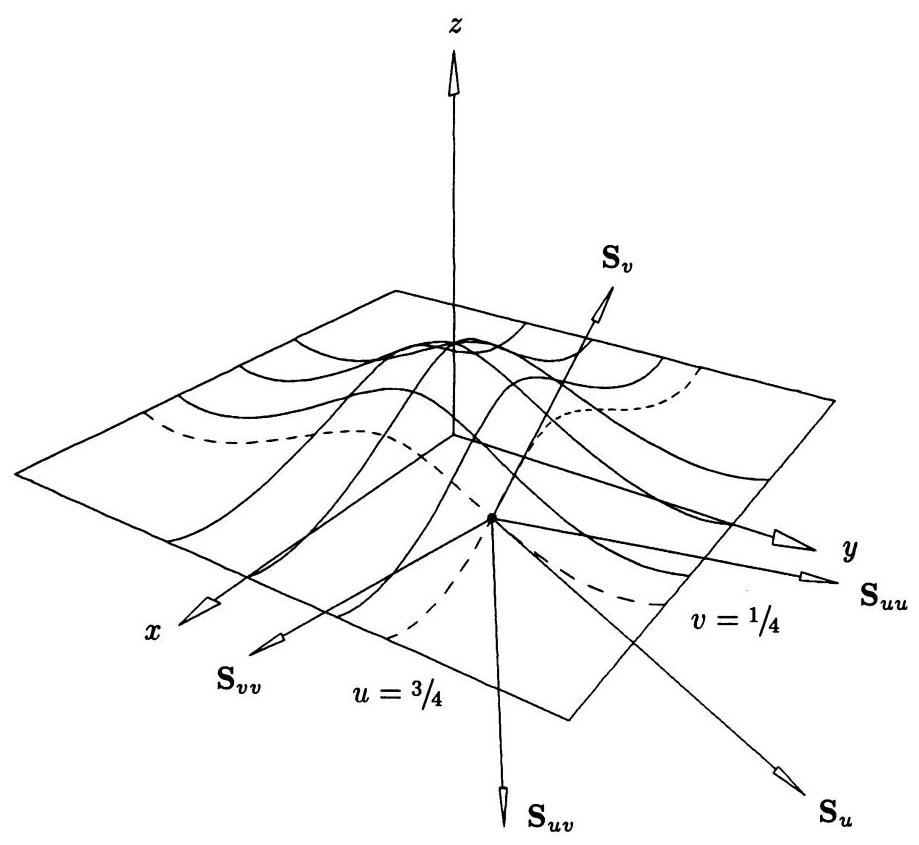
\includegraphics[max width=0.8\textwidth]{images/0193ba0d-ab19-7138-9798-cb281ce60de0_148_308_260_919_845_0.jpg}
\end{center}
\hspace*{3em} 

图 4.13. 在 \(u = 3/4\) 和 \(v = 1/4\) 处计算的双三次 NURBS 曲面的一级和二级偏导数。

\HRule

\hspace*{2em} for (i = 1; i<=k; i++)

\hspace*{4em} \{

\hspace*{4em} v = v - Bin[k][i]*wders[i][0]*SKL[k-i][l];

\hspace*{4em} v2 = 0.0 ;

\hspace*{4em} for (j=1; j<=1; j++)

\hspace*{5em} v2 = v2 + Bin[l][j]*wders[i][j]*SKL[k-i][l-j];

\hspace*{3em} v = v - Bin[k][i]*v2;

\hspace*{3em} \}

\hspace*{2em} SKL[k][l] = v/wders[0][0];

\hspace*{2em} \}

\}

\HRule

\section*{练习}

4.1. 设 \(U = \{ 0,0,0,1/3,2/3,1,1,1\}\) 和 \(\left\{  {{w}_{0},\ldots ,{w}_{4}}\right\}   = \{ 1,4,1,1,1\}\) 。使用 Cox-deBoor 递归公式 (公式 [2.5]) 和公式 (4.2)，计算五个二次有理函数 \({R}_{i,2}\left( u\right) ,0 \leq  i \leq  4\) 。这些函数的图形如图 4.5a 所示。假设 \(\left\{  {{\mathbf{P}}_{0},\ldots ,{\mathbf{P}}_{4}}\right\}   = \{ \left( {0,0}\right) ,\left( {1,1}\right) ,\left( {3,2}\right) ,\left( {4,1}\right) ,\left( {5, - 1}\right) \}\) 是 \({xy}\) 平面中的控制点。计算有理坐标函数 \(x\left( u\right)\) 和 \(y\left( u\right)\) ，表示在区间 \(u \in  \left\lbrack  {1/3,2/3}\right)\) 内的 \(\mathbf{C}\left( u\right)\) 。

4.2. 参考示例 Ex4.2 计算二次有理 Bézier 圆弧; 计算 \({\mathbf{C}}^{\prime \prime }\left( 1\right)\) 。

4.3. 设 \({\mathbf{C}}^{w}\left( u\right)  = \mathop{\sum }\limits_{{i = 0}}^{1}{N}_{i,1}\left( u\right) {\mathbf{P}}_{i}^{w}\) 为 \({xy}\) 平面中的一条线段，其中 \({\mathbf{P}}_{0} =\)  \(\left( {0,1}\right) ,{\mathbf{P}}_{1} = \left( {2,0}\right) ,{w}_{0} = 1,{w}_{1} = 3\) ，且 \(U = \{ 0,0,1,1\}\) 。推导出表示该线段的 \(x\) 和 \(y\) 坐标的有理函数，即 \(x\left( u\right)\) 和 \(y\left( u\right)\) ，其中 \(\mathbf{C}\left( u\right)  = \left( {x\left( u\right) ,y\left( u\right) }\right)\) 。使用公式 (4.9) 计算 \({\mathbf{C}}^{\prime }\left( 0\right)\) ，并使用公式 (4.8) 和 (3.9) 计算 \({\mathbf{C}}^{\prime \prime }\left( 0\right)\) 。然后设定 \({w}_{1} = 1\) 并重新计算 \(x\left( u\right) ,y\left( u\right) ,{\mathbf{C}}^{\prime }\left( 0\right)\) 和 \({\mathbf{C}}^{\prime \prime }\left( 0\right)\) 。

4.4. 设 \({\mathbf{S}}^{w}\left( {u,v}\right)  = \mathop{\sum }\limits_{{i = 0}}^{1}\mathop{\sum }\limits_{{j = 0}}^{1}{N}_{i,1}\left( u\right) {N}_{j,1}\left( v\right) {\mathbf{P}}_{i,j}^{w}\) ，其中 \(\left\{  {{\mathbf{P}}_{0,0},{\mathbf{P}}_{1,0},{\mathbf{P}}_{0,1},{\mathbf{P}}_{1,1}}\right\}   =\)  \(\{ \left( {0,0,1}\right) ,\left( {0,1,3}\right) ,\left( {2,1,1}\right) ,\left( {2,0,3}\right) \} ,\left\{  {{w}_{0,0},{w}_{1,0},{w}_{0,1},{w}_{1,1}}\right\}   = \{ 2,1,1,1\}\) ，且 \(U = V =\)  \(\{ 0,0,1,1\}\) 。推导出四个有理基函数 \({R}_{i,j}\left( {u,v}\right) ,0 \leq  i,j \leq  1\) ，以及曲面 \(\mathbf{S}\left( {u,v}\right)\) 的有理坐标函数 \(x\left( {u,v}\right) ,y\left( {u,v}\right)\) 和 \(z\left( {u,v}\right)\) 。

4.5. 从练习 4.4 中的 \({\mathbf{S}}^{w}\left( {u,v}\right)\) 推导出两个有理等参数曲线 \({\mathbf{C}}_{{u}_{0}}^{w}\left( v\right)\) 和 \({\mathbf{C}}_{{v}_{0}}^{w}\left( u\right)\) ，对于 \({u}_{0} = 1/3\) 和 \({v}_{0} = 1/2\) 。然后分别在 \(v = 1/2\) 和 \(u = 1/3\) 处评估曲线 \({\mathbf{C}}_{{u}_{0}}\left( v\right)\) 和 \({\mathbf{C}}_{{v}_{0}}\left( u\right)\) 。通过将 \(\left( {u,v}\right)  = \left( {1/3,1/2}\right)\) 代入在练习 4.4 中获得的有理坐标函数来检查结果。

4.6. 设 \({\mathbf{S}}^{w}\left( {u,v}\right)  = \mathop{\sum }\limits_{{i = 0}}^{1}\mathop{\sum }\limits_{{j = 0}}^{1}{N}_{i,1}\left( u\right) {N}_{j,1}\left( v\right) {\mathbf{P}}_{i,j}^{w}\) 为练习 4.4 中给出的曲面。由于 \({N}_{0,1}\left( {1/2}\right)  = {N}_{1,1}\left( {1/2}\right)  = 1/2\) ，因此得出

\[
{\mathbf{S}}^{w}\left( {\frac{1}{2},\frac{1}{2}}\right)  = \frac{1}{4}\left( {{\mathbf{P}}_{0,0}^{w} + {\mathbf{P}}_{0,1}^{w} + {\mathbf{P}}_{1,0}^{w} + {\mathbf{P}}_{1,1}^{w}}\right)  = \left( {1,\frac{1}{2},\frac{9}{4},\frac{5}{4}}\right)
\]

计算 \({\mathbf{S}}_{u}\left( {1/2,1/2}\right) ,{\mathbf{S}}_{v}\left( {1/2,1/2}\right) ,{\mathbf{S}}_{uv}\left( {1/2,1/2}\right) ,{\mathbf{S}}_{uu}\left( {1/2,1/2}\right)\) 。



\clearpage

\end{document}


